\section{Implementierung}
Im folgenden Kapitel betrachten wir die Implementierung des Prototypen.


\subsection{OpenSource}
Der Quellcode des entwickelten Prototypen ist auf GitHub\footnote{\url{https://github.com/AsureNetwork/asure-dapp}} veröffentlicht und kann unter der ISC Lizenz\footnote{\url{https://github.com/AsureNetwork/asure-dapp/blob/master/LICENSE}} im Rahmen weiterer Softwareprojekte genutzt werden.

\paragraph*{}
Der Prototyp steht unter der Adresse \url{https://dapp.asure.io/} zum testen zur Verfügung. 

\subsection{Anwendungsfälle}
Das deutsche gesetzliche Rentensystem basiert im Kern auf der Rentenformel, durch welche die Höhe der Rentenzahlung jedes Rentenempfänger ermittelt wird. Durch eine Vielzahl von Sonderregelungen gestaltet sich das Rentensystem jedoch sehr komplex, weshalb eine vollumfängliche Abbildung des Systems im Rahmen eines Prototypen nicht sinnvoll ist. Stattdessen wurden einige Anwendungsfälle ausgewählt, und im Umfang an die Anforderungen eines Prototypen angepasst.

\paragraph{}
Alle Anwendungsfälle zusammen, bilder den kompletten Zyklus eines Rentensystems ab - Von der Zahlung der Beiträge, bis zur Zahlung der Renten.

\paragraph{}
Die Anwendungsfälle sind wie folgt definiert:

\begin{compactenum}
\item Als Benutzer möchte ich mich als Versicherter registrieren.
\item Als Beitragszahler möchte ich mein geplantes Renteneintrittsdatum festlegen.
\item Als Beitragszahler möchte ich jeden Monat in das Rentensystem einzahlen.
\item Als Rentner möchte ich jeden Monat eine Rente auszahlen.
\item Als Versicherter möchte ich eine Übersicht über meine Beiträge / Rentenzahlungen angezeigt bekommen.
\item Als Versicherter möchte ich alle Aktionen via Smartphone Anwendung durchführen.
\item Als Administrator möchte ich das Backend (Smart Contracts) auf dem öffentlichen Ethereum Testnet bereitstellen.
\end{compactenum}


\subsection{Deutsche Rentenformel}
Für die Berechnung der Höhe der Renten wurde die deutsche Rentenformel (Siehe \ref{eq:rentenformel}) verwendet.
\\
Dabei wurde im Rahmen des Prototypen nur die Berechnung der Entgeltpunkte (EP) implementiert. 
\\
Der Wert für den Zugangsfaktor (ZF) als auch für den Rentenartfaktor (RAF) ist immer 1. Hieraus resultiert, das die berechneten Renten immer einer Rente wegen Alters und regulären Rentenbeginn entsprechen.
\\
Auch der Wert für den aktuelle Rentenwert (aRW) ist statisch und beträgt immer \EUR{29}. Der entsprechende Quellcode für die Ermittlung des aktuellen Rentenwerts (aRW) ist so strukturiert, das dieser pro Jahr im System mittels einer Lookup Tabelle hinterlegt werden kann.

\begin{equation*} \label{eq:rentenformel}
Rente_{mtl} = EP \cdot ZF \cdot RAF \cdot aRW
\end{equation*}

\begin{compactitem}
\item \textbf{Rente\textsubscript{mtl}} ist die monatliche Bruttorente in Euro
\item \textbf{EP} ist die Summe der Entgeltpunkte aufgrund des Versicherungsverlaufs
\item \textbf{ZF} ist der Zugangsfaktor
\item \textbf{RAF} ist der Rentenartfaktor
\item \textbf{aRW} ist der aktuelle Rentenwert in Euro
\end{compactitem}


\subsection{Anwendungsarchitektur}
Die Benutzeroberfläche des Prototypen wurde als Progressive Web App (PWA) entwickelt und für die Verwendung auf Mobilgeräten optimiert. Ein Webserver liefert die Webanwendung mittels HTTP/HTTPS an den Browser.
\\
Das Backend bildet ein Smart Contract-System, welches auf dem öffentlichen Ethereum Testnetz Rinkeby gehostet wird und mit dem die Benutzeroberfläche mittels HTTP/WebSockets kommuniziert. Für den Zugriff auf ein Ethereum Netz wird ein Ethereum Knoten (ggf. auch ein Ethereum Cluster für Ausfallsicherheit) benötigt. Im Rahmen des Prototypen verwenden wir hierzu Hosting Provider wie Infura und Cloudflare, welche entsprechende Ethereum Knoten hosten und zur Verfügung stellen.\footnote{Die Dezentralisierung und somit das Betreiben eigener Ethereum Knoten ist ein entscheidener Vorteil der Blockchain-Technologie. Durch die Verwendung von gehosteten Ethereum Gateways (Infura / Cloudflare) wird dieser Vorteil nicht genutzt.}

\begin{figure}
    \centering
    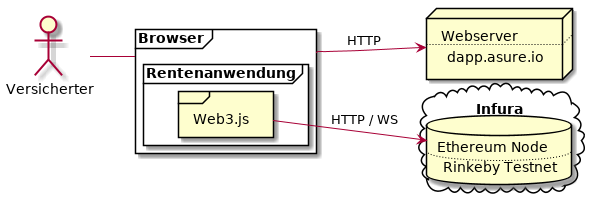
\includegraphics[width=6.0in]{images/components.png}
    \caption{Komponenten des Prototyps}
\end{figure}


\subsection*{Smart Contract Entwicklungswerkzeuge}
Im Rahmen der Backend Entwicklung wurde ein Smart Contract System für die Ethereum Blockchain entwickelt. Für die Entwicklung kamen die folgenden Tools zum Einsatz:

\paragraph*{Solidity} ist eine objektorientierte, anwendungsspezifische höhere Programmiersprache mit einer JavaScript-ähnlichen Syntax zum Entwickeln von Smart Contracts für Blockchain-Plattformen wie Ethereum oder Tron.\\ %TODO cite
Sämtliche Smart Contracts des Prototypen wurden in Solidity programmiert.

\paragraph*{OpenZeppelin Contracts} ist ein Framework aus modularen, wiederverwendbaren und sicheren Smart Contracts für das Ethereum-Netzwerk, geschrieben in Solidity.

\paragraph*{Truffle} ist ein Entwicklungsframework für Ethereum. Es bietet u.a. Funktionen für das Erstellen von automatisierten Tests, Deployments und Migrationen von Smart Contracts. Zudem können mit Truffle verschiedenen Ethereum Netwerke wie z.B. ein lokales Entwicklungsnetz, oder das öffentliche Ethereum Testnetz Rinkeby verwaltet werden.

\paragraph*{Ganache} ist eine Ethereum Software, welche speziell für die Entwicklung von Smart Contracts entwickelt wurde. Ganache bietet Erweiterungen um z.B. innerhalb von Unit Tests die Uhrzeit zu Manipulieren und somit auch uhrzeitabhängige Funktionalitäten zu testen.

\paragraph*{Infura} bietet einen skalierbaren API-Zugriff auf öffentliche Ethereum-Netzwerke.


\subsection{Smart Contract Architektur}

\begin{figure}[H]
    \centering
    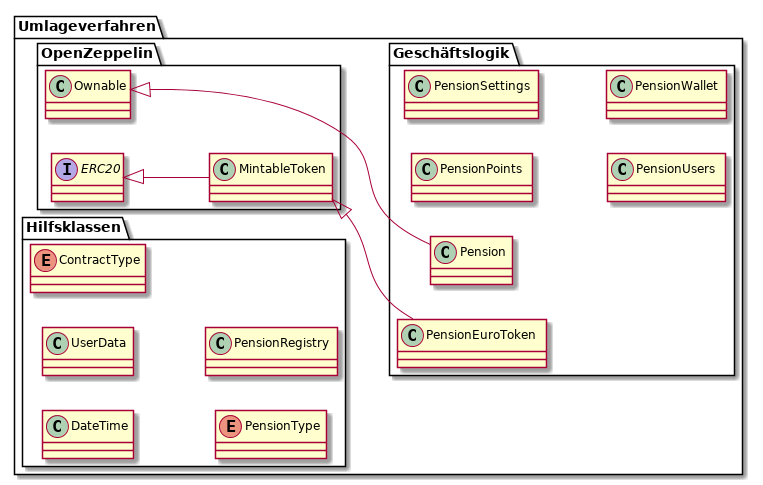
\includegraphics[width=6.0in]{images/classdiagram-smartcontracts.png}
    \caption{Smart Contracts Übersicht}
    \label{fig:asure_architecture}
\end{figure}


\paragraph*{PensionUsers:} Registrierung und Verwaltung von Benutzern und deren Stammdaten.

\paragraph*{PensionWallet:} Beitrags-, und Rentenzahlungen - Verwaltet sämtliche Geldmittel.


\paragraph*{PensionPoints:} Datenhaltung Beitragszahlungen und Entgeltpunkte.

\paragraph*{Pension:} Berechnung der Höhe der Rentenzahlungen.

\paragraph*{PensionSettings:} Verwaltung diverser Parameter (z.B. Rentenartfaktor (RAF) / Rentenwerte (aRW)).

\subsubsection{Anwendungsfall: Als Beitragszahler möchte ich jeden Monat in das Rentensystem einzahlen}

\begin{figure}[H]
    \centering
    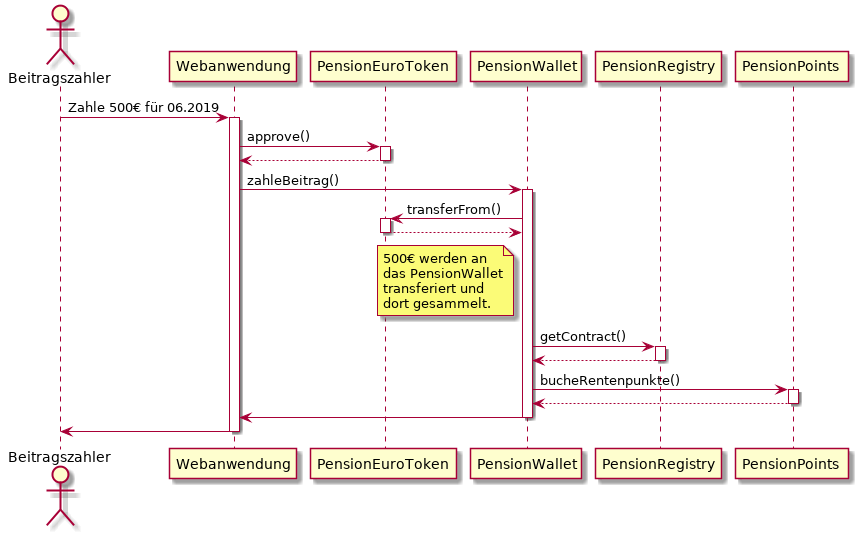
\includegraphics[width=6.0in]{images/usecase-pay.png}
    \caption{Sequenzdiagram: Beitragszahlung}
    \label{fig:asure_architecture}
\end{figure}

\subsubsection{Anwendungsfall: Als Rentner möchte ich jeden Monat eine Rente auszahlen}

\begin{figure}[H]
    \centering
    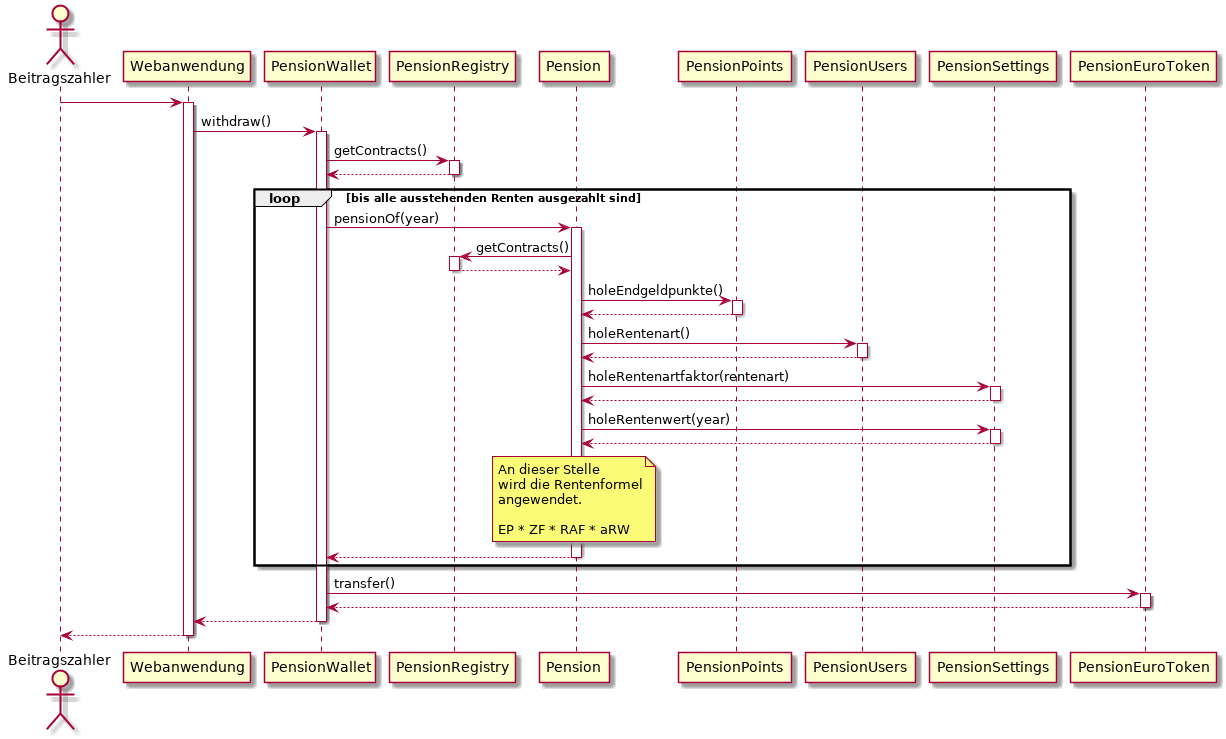
\includegraphics[width=6.0in]{images/usecase-payout.png}
    \caption{Sequenzdiagram: Rentenzahlung}
    \label{fig:asure_architecture}
\end{figure}